\begin{frame}\begin{center}
		\LARGE\textit{Individual Heterogeneity}
\end{center}\end{frame}
%-------------------------------------------------------------------------------
%-------------------------------------------------------------------------------
\begin{frame}
	Individual-specific Benefit of Treatment
	\begin{align*}
		Y_1 - Y_0 = (\mu_1(X) - \mu_0(X)) + (U_1 - U_0)\\
	\end{align*}
	\textbf{Sources of Heterogeneity}
	\begin{itemize}\setlength\itemsep{1em}
		\item Difference in Observable Characteristics
		\item Difference in Unobservable Characteristics\medskip
		\begin{itemize}\setlength\itemsep{1em}
			\item  Uncertainty
			\item Private Information
		\end{itemize}
	\end{itemize}
\end{frame}
%-------------------------------------------------------------------------------
%-------------------------------------------------------------------------------
\begin{frame}
	\begin{figure}\caption{Distribution of Benefits}
		\scalebox{0.35}{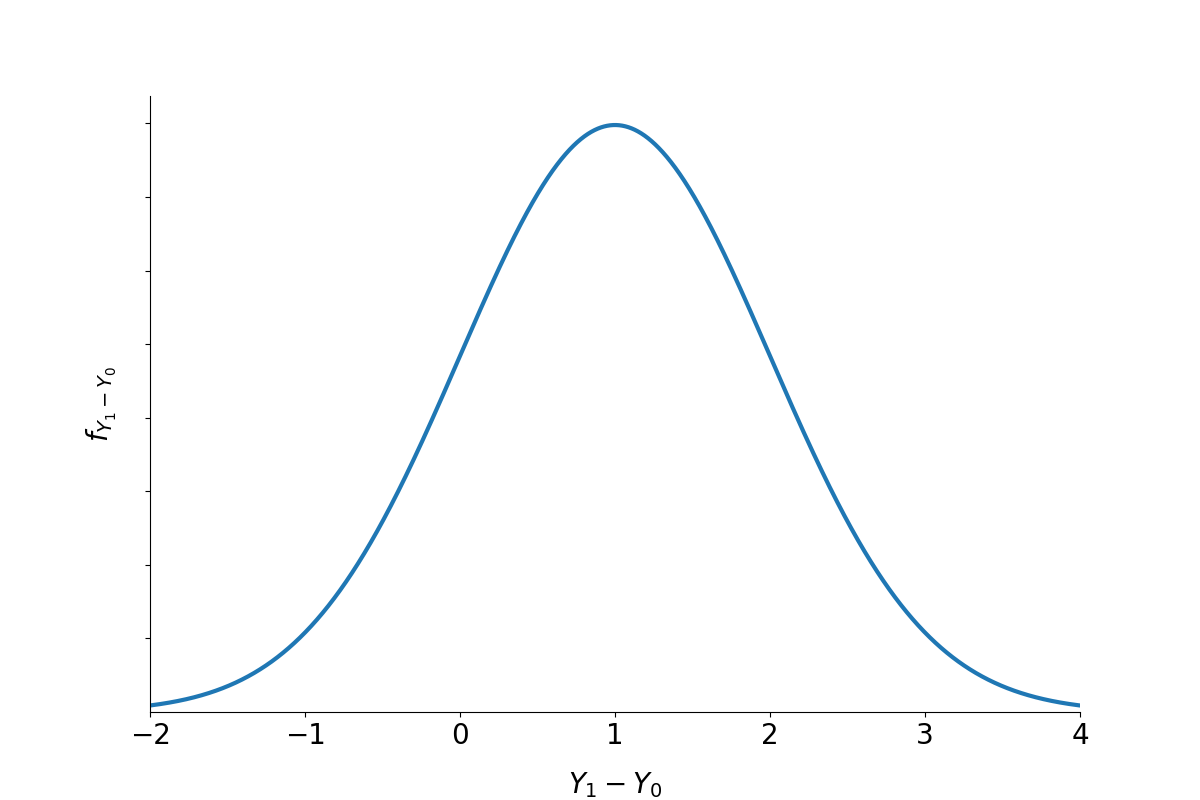
\includegraphics{fig-treatment-effects-benefits.png}}
	\end{figure}
\end{frame}
%-------------------------------------------------------------------------------
%-------------------------------------------------------------------------------
\begin{frame}
	\textbf{Essential Heterogeneity}\vspace{0.5cm}	
	\textbf{Definition:} Individuals select their treatment status based on
	gains unobservable by the econometrician. More formally,	
	\begin{align*}
		Y_1 - Y_0 \notindep D\quad \mid X = x.
	\end{align*}	
	\(\Rightarrow\) consequences for the choice of the estimation strategy	
\end{frame}
%-------------------------------------------------------------------------------
%-------------------------------------------------------------------------------
\begin{frame}
	\begin{figure}\caption{Conditional Expectation and Essential Heterogeneity}
		\scalebox{0.35}{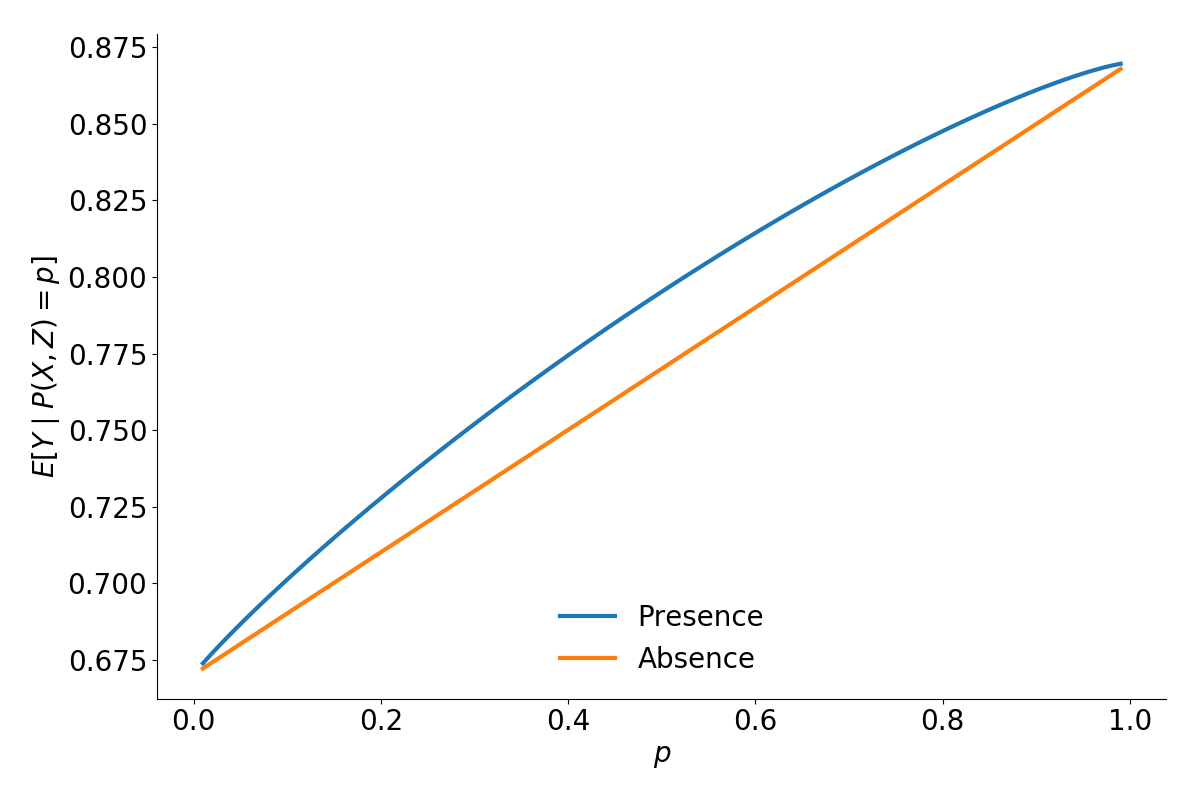
\includegraphics{fig-eh-conditional-expectation}}
	\end{figure}
\end{frame}
